\documentclass[a4paper]{article}
\usepackage[utf8]{inputenc}
\usepackage[english]{babel}
\usepackage{amsmath}
\usepackage{amsfonts}
\usepackage{amssymb}
\usepackage{graphicx}
\usepackage{geometry}
\usepackage{footnote}
\usepackage[section]{placeins}
\usepackage{pdfpages}

\makesavenoteenv{tabular}


\title{PFR - Project Final Report}
\author{Team 2}

\begin{document}
\begin{titlepage}
\newgeometry{left=2cm,top=1cm,right=2cm}
\newcommand{\HRule}{\rule{\linewidth}{0.5mm}}

\begin{minipage}{0.5\textwidth}
\begin{flushleft} % Responsible persons, write on separate lines
\textit{Responsible for this document:}\\
Emma Albertz \\
Linnéa Claesson
\end{flushleft}
\end{minipage}
~
\begin{minipage}{0.4\textwidth}
\begin{flushright}
PUSS154219 v0.1 
\today
\end{flushright}
\end{minipage}\\[3cm]

\centering
\textsc{\LARGE Team 2}\\[0.5cm]

\HRule \\[0.4cm]
{ \huge \bfseries Project Final Report}\\[0.4cm] % Title of your document
\HRule \\[1.5cm]

\vfill
\begin{flushleft}
%Authors, write on separate lines
\textit{Authors of this document:}\\
Emma Albertz \\
Linnéa Claesson\\
Jacob Mejvik
\end{flushleft}



\end{titlepage}
\pagenumbering{gobble}



%\begin{center}
%\textit{\large Version History}
%
%    \begin{tabular}{ | l | l | l | p{5cm} |}
%    \hline
%    \textbf{Version} & \textbf{Date} & \textbf{Responsible} & \textbf{Description} \\ \hline
%    1.0 & 150916 & EA, LC & Baseline\\ \hline
%    \end{tabular}
%\end{center}



\setcounter{tocdepth}{2}
\tableofcontents
\newpage
\pagenumbering{arabic}

\section{Reference Documents}
\begin{enumerate}

\item[Ref1] Veckoschema PUSS154251

\item[Ref2] Gantt schema PUSS154252 

\end{enumerate}


\section{Introduction}
At the time this report is being written, the product is not completely finished. This document aims to analyse and evaluate the team's continuous work and the system to be delivered. Estimations on the last week's work and expected quality of the finished product have therefore been made. 

Metrics data has been collected throughout the work, which is presented in section~\ref{sec:metr} and evaluated in section~\ref{sec:meval}.

A questionnaire was sent out for all team members to fill out. The replies to this questionnaire is evaluated and presented in section~\ref{sec:teval}. Suggestions for improvement based on these replies are then presented in section~\ref{sec:impr}.

The team has during the work been divided into four subgroups with different responsibilities:

\begin{description}
\item[Project Managers] Two people responsible for the entire project, planning and making sure everything is delivered on time and up to standard.
\item[System Architects] Responsible for the technical part of the project and communications between the developers and testers. Consisted of three people, one of whom was system manager.
\item[Developers] Eight developers have been responsible for the implementation of the application.
\item[Test Group] Six testers have been responsible for testing the developed system, one of whom has been acting as test manager.
\end{description}

The shared opinion within the team is that this has been a well executed project where everyone has contributed to their part to make sure that the delivered system is up to standards with the customer's request.  

%-------------------------- Project Metrics --------------------------------------%
% Historisk överblick över projektet
% Vad är det som har hänt? Siffror, tabeller och diagram. Jämförelser och uppvisande av data. 
\newpage
\section{Project Metrics}
\label{sec:metr}

\begin{figure}
\centering
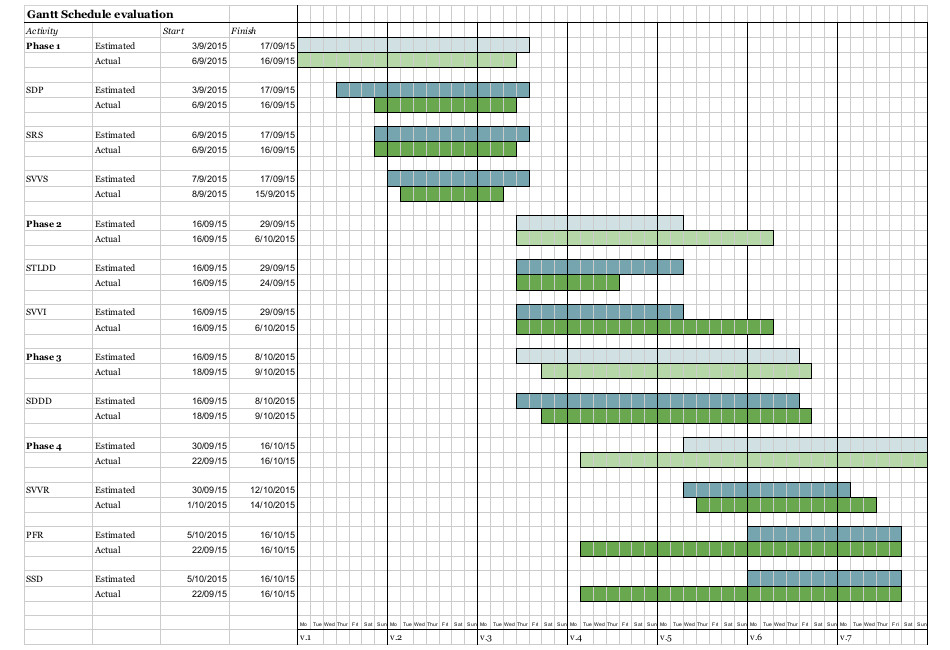
\includegraphics[width=0.9\textwidth]{gantt.jpg}
\label{fig:gantt}
\caption{Comparison between the estimated Gantt schedule and the outcome.}
\end{figure}

\begin{figure}[h!]
\centering
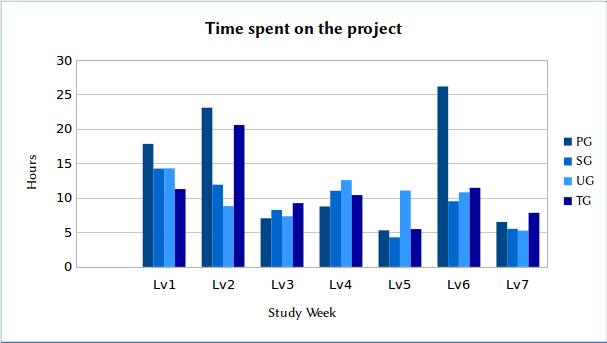
\includegraphics[width=0.7\textwidth]{time.jpg}
\label{fig:time}
\caption{Average time spent per week fand person of each subgroup.}
\end{figure}



\begin{figure}[h!]
\centering
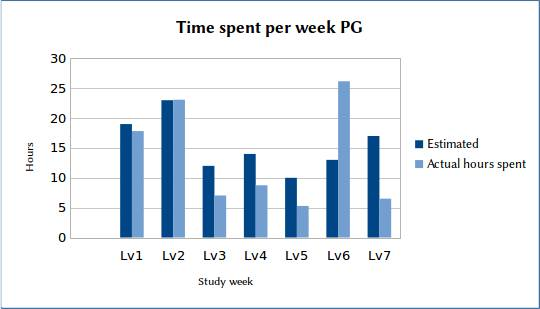
\includegraphics[width=0.7\textwidth]{pg.jpg}
\label{fig:pg}
\caption{Average estimated and actual amount of hours spent by project managers per week.}
\end{figure}

\begin{figure}[h!]
\centering
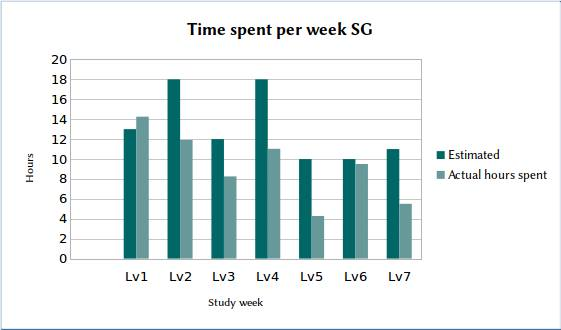
\includegraphics[width=0.7\textwidth]{sg.jpg}
\label{fig:sg}
\caption{Average estimated and actual amount of hours spent by system architects per week.}
\end{figure}

\begin{figure}[h!]
\centering
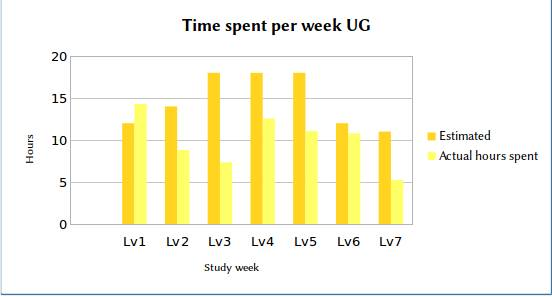
\includegraphics[width=0.7\textwidth]{ug.jpg}
\label{fig:ug}
\caption{Average estimated and actual amount of hours spent by developers per week.}
\end{figure}

\begin{figure}[h!]
\centering
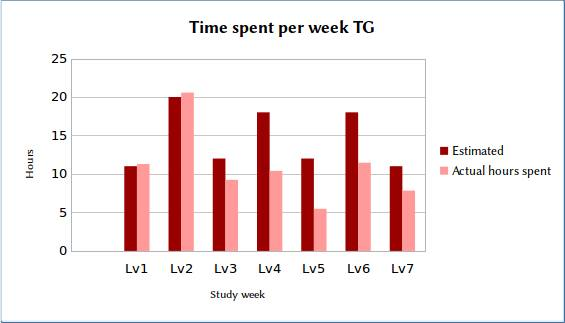
\includegraphics[width=0.7\textwidth]{tg.jpg}
\label{fig:tg}
\caption{Average estimated and actual amount of hours spent by tester per week.}
\end{figure}



\begin{figure}[h!]
\centering
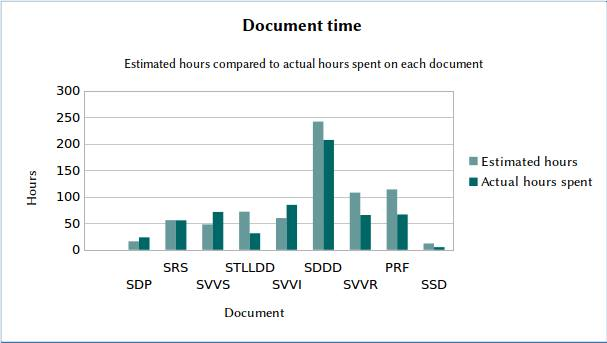
\includegraphics[width=0.7\textwidth]{doc.jpg}
\label{fig:doc}
\caption{Estimated hours compared to actual hours spent on each document.}
\end{figure}

\begin{figure}[h!]
\centering
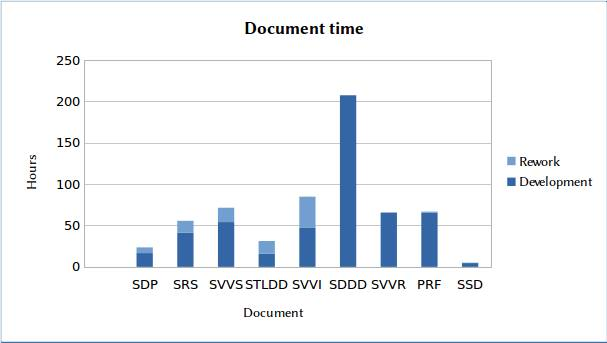
\includegraphics[width=0.7\textwidth]{dev-re.jpg}
\label{fig:dev-re}
\caption{Hours spent on each document divided into development and rework.}
\end{figure}


\begin{table}[h!]
\centering
\caption{Table caption}
\begin{tabular}{|l|c|c||c|c|}
 \hline
\multicolumn{3}{|c||}{\textbf{Estimated}} & \multicolumn{2}{|c|}{\textbf{Result}}\\ \hline \hline
\textbf{Activity} & \textbf{h total} & \textbf{h/person} & \textbf{h in total} & \textbf{h/person} \\ \hline
SDP & 16 & 8 & 24 & 12 \\ \hline
SRS & 56 & 8/4 & 56 & 13/2 \\ \hline
SVVS & 48 & 8 & 71 & 12 \\ \hline
STLDD & 72 & 8/6 & 31 & 10\\ \hline
SVVI & 60 & 10 & 85 &14\\ \hline 
SDDD & 242 & 25/14 & 207 & 26 \\ \hline
SVVR & 108 & 18 & 36 & 6\\ \hline
PRF & 114 & 6 & 67 & 25/1\\ \hline
SSD & 12 & 6 & 5 & 3 \\ \hline

\end{tabular}
\label{table:time}
\end{table}

Om du vill referera till tabellen ovan skriv "In table~\ref{table:time} bla bla bla".

\FloatBarrier
%------------------------- Project Evaluation -----------------------------------%
% Utvärdering av vad som gick bra/dåligt
% Varför ser datan ut som den gör? Analys av de siffror man samlat in. Ex fasernas tidsåtgång, dokumentens antal timmar (UIFO), gruppernas timmar / vecka
\section{Project Evaluation}


\subsection{Evaluation of Project Metrics}
\label{sec:meval}

Introtext

\subsubsection{Ny sektion}

\subsubsection{Gantt Schedule}
Overall, the dates set for the phases and the documents in the project has been followed with only smaller deviations. All according to the time plan made in the beginning of the project. However a few bigger deviations have occurred.

From the way it looks in the Gantt chart, SVVI took approximately a week longer than expected. This caused an extension of phase two. The reason for this was an administrative error. The document was actually ready within the planned time but was by mistake not put into baseline immediately. 

Phase four started earlier than planned since project leaders found it appropriate to start preparing for the final reports as much as possible in advance. This to ease the workload in the final stage of the project as much as possible.


\subsection{Evaluation of Delivered System and Performance of Team}
\label{sec:teval}
As part of the project evaluation, a questionnaire was sent out for all team members to fill out. The replies to this questionnaire were used to evaluate the team's performance during this project and are presented in this section. 

Overall, the general consensus has been very positive and everyone seems very satisfied with both their own and the team's contribution to the project.


%----------------------- Time Planning ---------------------------------%

\subsubsection{Time Planning}
The scheduling and time planning of the project have received very positive response from the team. The project managers put a lot of time into working out a reasonable schedule that would also make sure that the project was delivered prior to external commitments the team members had at the end of the time period scheduled for this project. This lead to some tight deadlines, but the team was motivated to meet them due to it being to their personal advantage. At the time of this report being written, the deadlines have all been successfully met. 

The Weekly Schedule and Gantt Chart, Ref1 and Ref2 respectively, produced by the project managers could have been referred to more often throughout the project. Overall though, the team members have stated that they have known what they needed to do and when they needed to do it. It has been stated that the pace of the project has been high, but that it has been good so the project can be finished before the external commitments previously mentioned. 

Once a week a project meeting has been held where all team members have been expected to attend. The group meetings have been a great help in keeping the members of the team updated on upcoming deadlines and providing a chance for the project managers to make sure that the team is where it should be. Both the attendance and replies to the questionnaire have shown that these meetings were greatly appreciated and well carried out.

The developers did not have as much work in the beginning as the others, but this changed once they started implementing the code and they had to put in a couple of weekends to finish. This seems to have worked fine, even though there were some who could not attend these weekend group sessions.

The testers were sometimes dependent on the system architects to finish their reports before the testers could finish their own, which added a bit of pressure at the final stages of the writing of the reports. A slightly earlier deadline was often set for the system architects than the testers, but they were not given much extra time either since this would affect the system architects negatively.


%---------------------- Work Distribution ------------------------------%

\subsubsection{Work Distribution}

A responsible person for each task was decided at the group meetings. The division of the larger tasks into smaller has then been done internally within each subgroup, sometimes in collaboration with other subgroups (such as system architects and developers). This system has worked very well for this project. The project managers have always known who to talk to about each specific task to make sure everything is coming along as expected and that person can in turn make sure everyone within his or her subgroup is making the progress they should. 

The responsibilities between the two project managers were easily shared. They had prior knowledges that complemented each other well and therefore found natural ways to divide the tasks between them. They regularly met to plan meetings and deadlines together and update each other on their respective tasks' progresses. 

The same arrangements were made within the system architects group. Some had more technical skill sets and therefore took on greater responsibilities in those areas, whereas others had more experience in working with this kind of project were a lot of reports were to be produced at a certain standard and could therefore take on more responsibility in those areas. 

Even though one of the system architects has acted as system manager, the organisation within their group has been very flat. They have met often to make sure everyone is on the same page with everything and they have all truly contributed to this project.

It was a bit unclear in the beginning how much responsibility the system architects should have. This could (and should) have been evaluated better and made clear from the beginning by the project managers, to avoid confusion. Overall though, they have known what needed to be done and no major issues arose due to this.

The developers have worked in pairs with their assignments. Most of them had no previous experience with Android development. Working in pairs really helped overcoming something that at first might have seemed very difficult, but still making each member responsible for a part of the project. The division of what each pair should do came as a suggestion from the system architect group, who had prior experience with Android development and knew approximately how much time each task should take. There was one part of the project that was slightly larger than the others and the pair working on it had some difficulties, but the system architects stepped in and offered help so they could finish on time.

Overall the distribution of work among the developers has worked fine. Some of them have not seemed to prioritise this project and instead go and work on other things (everyone in the team has other commitments). This slowed down the development of the product, which could have been finished at an earlier stage had not some members postponed their tasks to the last minute. This was not a real problem though, considering the deadlines were met. 

The work among the testers has also worked very well. There have been some inequalities in work load due to the fact only a couple of people within the group had previous knowledge of LaTex and GitHub. This meant that they had to pull a larger weight in fixing problems for the entire group.



%----------------- Communication -----------------------------%

\subsubsection{Communication}
One thing in particular that has worked very well throughout the project is the communication within the team, within each subgroup and also between the subgroups of the team. The developers have reported that there has been exceptional communications between them and the system architects, who have been a great help and contribution in the developers' progress and success.

A big contribution to the communication within the group functioning so well has been the weekly project group meetings. The meetings have been held at the same time and place each week, to avoid confusion and people missing meetings due to unclear scheduling. 

At these meetings information to the team was given from the project managers and each subgroup has updated the rest of the team on their current status and progress. The questionnaire and the attendance showed that these meetings were appreciated and a great help in keeping track of what needed to be done and when. Who would be responsible for what part of the project, how issues should be handled and deadlines were set at these meetings.

The group meetings were also a place for discussion and gave an opportunity to ask the other team members questions and raise concerns. It also helped keep the project managers updated in how the work was going in each subgroup and making sure deadlines could be met.

Meeting protocols were constructed for each meeting and posted afterwards both on the team's joint Drive and Git repository, to be available for later reference and/or read by those who might have missed a meeting.

The subgroups have also had their own internal group meetings whenever they needed, to discuss topics not needed to be addressed at the larger group meetings. These topics include e.g. division of assignments and internal deadlines.

Information that could not wait to be brought up at the project meeting has been sent out by email. A Facebook group has also been used as a means for fast but secondary communications.

There was a discussion at the beginning of the project on whether or not to use Piazza as a means of communication within the group. Since it was not available from the start of the project other alternatives were used instead and by the time Piazza was working, these alternatives had already been established. There has been a difference of opinion within the group whether or not Piazza should have been used during the project and this should be evaluated for future projects.

Communications with the customer and experts have not been as well functioning as communications within the team. Especially the testers have reported that they could have avoided some, in hindsight, simple issues by contacting the experts at an earlier stage of the project. The project managers and/or the system architects could also have had a better dialogue with the customer to continuously make sure that the system being developed was in fact the system ordered. The acceptance test has still not taken place at the time when this report is being written, but two formal reviews have been held with the customer prior to the acceptance test to make sure that the right system is being developed.


%---------------- Knowledge -------------------------------------%

\subsubsection{Experience and Knowledge}
Both among the project managers and the system architects, the members had different sets of knowledge when coming into this project. Some had more technical skills, such as prior experience with the tools used (GitHub, LaTex and Android Studio) whereas others had more experience with this kind of administrative work and report writing. In both groups this worked very well, since they complemented each other and made the groups more knowledgeable as a whole than each individual. Everyone could make valuable contributions to the project.

Not many among the developers had previously worked with Android development, LaTex and/or GitHub. Since the external training that was provided came far too late in the process, the system architects had to step in and take a large part in training the developers in these areas. The external training also only covered Android development and not the other tools used for this project.

During the development of the product, the developers often chose to meet up and work together, even though the task was divided into smaller ones among them. This meant they could collaborate and help each other with problems. In addition to this, they could keep an open dialogue and everyone knew at what stage everyone else was at.

Som issues arose from the fact that not many among the developers had any previous experience with programming in a larger group. People would push code to git that could not be compiled, leading to problems for the rest of the group. A lot of time was wasted in dealing with these situations.

As previously mentioned, there was a large difference in prior working experience with the tools used (LaTex and GitHub) within the test group . This led to some doing a lot more work than the others when it came to solving problems generated by the tools they used, since they were the only ones who knew how to do it.


%------------------ Technical Issues ---------------------------------%

\subsubsection{Technical Issues}

Some technical issues were encountered during the work on this project, most of which were introduced outside of the group's control.

Bugs were discovered in the back end product, which the group had no control over or ability to fix and therefore had to work around.

Android Studio was not properly installed and available on the computers provided for this project, which meant that the developers had to use their own computers and install Android Studio on them. This caused issues for some members of the group who only owned stationary computers and therefore could not work together with the rest of the group. Some installation issues were also encountered but eventually fixed, but unnecessary time was spent on this process that otherwise could have been spent on development of the product.

The team was also supposed to use Piazza as a means of communications, both within the group and with the experts and customers. Piazza was not made available from the beginning of the project and therefore other tools were established before the team could start using Piazza and its advantages were then lost.

E-puss was also not available from the beginning, which caused some discomfort but no lasting consequences.


\subsubsection{Documents and Final Product}
When the questionnaire was sent out and this report written, the product was not yet completely finished. Estimations have therefore been made with respect to how satisfied the team will be with the final product. A lot of confidence was shown throughout the replies of the questionnaire, that the developers will be able to present an application that reflects the team's efforts and hard work. 

The project managers are very satisfied with the quality of the documents so far delivered and believe without a doubt that with the help of the system architects and testers, the developers will be able to finish the application on schedule and to a satisfactory result.

The system architects have made sure that the Software Top Level Design Document (STLDD) has been followed. As always, things could have been implemented differently but at the time of the writing of this report, everything looks good and the system architects have faith in the developers ability to deliver the product ordered, based on the competence and hard work they already have put into it.  

The system architects are also satisfied with their own work and results. They have put a lot of effort into this project and have made sure that the developers have had everything they needed throughout the development of the product.

Since there has been a very high level of competence among the system architects, the system manager would have liked to see an even higher level on the documents they delivered. The time and fast pace have been limiting factors for this, though. 

The developers started to implement the code in parallel with the STLDD being written. This caused some issues when changes were made in STLDD that affected the code, but overall the product could be finished faster in doing so. 

Most of the documents are based on templates provided by the customer, to make sure they follow a certain format and standard. This has been really helpful, since it has been clear from the beginning what the customer has expected.

There has been some dependence between some of the documents the team has delivered. It has been up to the system architects to manage this and make sure that everyone concerned has gotten the information they need to update their documents according to the changes made in another. A lot of work has been put into this and the other groups have seemed satisfied with the result. There were some miscommunication in the beginning of this process though, concerning documents produced by the system architects that affected documents produced by the testers. This was partly due to the project managers not communicating clearly from the beginning how these situations should be handled. 


The developers are pleased with their contribution to the product. The main issues they have encountered in the development stage have been due to the back end and sensor not working properly. This has been out of their control, but a list of bugs in the back end has been delivered to the customer. 

\subsubsection{Problem Handling}

The procedure for handling problems in the project has been very systematic. When a problem has been detected a problem report has been filed. Upon receiving a problem report the Change Control Board have investigated the problem, reviewed relevant documents and found a solution. Once a solution had been specified the responsibility to implement the changes was assigned and a deadline, usually within one day, specified. The process for handling problems has worked very well throughout the entire project. 

The filed problem reports have generally been highly relevant, describing issues that significantly impacts the projects ability to deliver a high quality product with consistent documents. For this reason, at the time of writing, all filed problem reports have been fully or partially accepted. In case of a partial acceptance the reason for deviation has usually been to keep a consistent and logic structure throughout all documents.

It should however be noted that the administrative load connected with handling problems has been high in comparison to the problem itself. This was anticipated, but in retrospect the load has been even higher than expected. The main reason for this is the rigorous procedure in connection with a desire to handle problem reports frequently and give quick feedback to relevant subgroups in order to shorten cycle times. At times this has meant that the Change Control Board has been forced to prioritize and had it not been for a well structured division of labour, they would have been hard pressed to deliver.

Furthermore, it has been noted that problem reports have had a tendency to occur more frequently towards the end of the project when the product nears completion. Problems that were injected later also tended to cause more widespread changes as more documents were set in baseline.

The problems that have occurred can mainly be divided into two categories, the first category being problems related to a mismatch between the STLDD and the SDDD. Some of these problem reports could have been avoided with a more thorough STLDD from the start. However, the changes have been of a minor character and the overall architecture has hardly been modified at all. With the benefit of hindsight, possibly the original design was somewhat overworked, containing a few unnecessary classes, in relation to the size of the application.

The second category is related to the back end. Changes had to be made due to the fact that the back end lacked basic functionality, such as being able to give accurate error messages, or that the functionality of the back end had been misunderstood in the early phases of development. Typically these errors propagated through several documents giving rise to various changes. Most of these issues were exceedingly hard to foresee and also resulted in multiple revisions in order to work around the constraints enforced by the back end.

In conclusion the problem handling has worked very well in terms of following the process, but has been quite labour intensive. Possibly some problem reports could have been avoided but the majority could not realistically be foreseen given the development model used. 

%------------------------ Suggestions for Improvement ---------------------------%
% Förbättringsförslag
% Hur ska man göra för att förbättra de positiva trenderna och få bort de negativa? Processförbättring mm.
\section{Suggestions for Improvement}
\label{sec:impr}

Even though the progression of this project has been a very good experience for all team members, there is always room for improvement and things that could have been done differently.

\subsection{Development}
One of the largest issues that came up was the lack of previous experience among the developers. The external training offered should be held at a much earlier stage than it was, which would have spared the system architects a lot of work. The developers could also themselves have taken responsibility in getting the knowledge and experience they knew they would need, especially since they did not have a lot of other assignments in the beginning of the project. The lack of knowledge was also known to the project managers and system architects. In hindsight it would have been a good idea if they had encouraged the developers more earlier in the project to retrieve the knowledge they would later need. They could have provided the developers with tutorials they could do to get the basics of Android development down and set a deadline for when this should be done. Instead, the system architects had to take on all this responsibility themselves in the beginning of the development phase. 

The project managers feel that they could have had a more present role in the development stage of the project, e.g. attending some of the meet ups the developers had, and not just rely on the information received at the project meetings once a week. 

\subsection{Documents and Administration}
The administrative part of the project was very large in comparison to the size of the developed system. A lot of time and effort was spent on producing the right documents and make sure that they kept a certain standard. This should be evaluated in the future to make sure that the time spent here is appropriate to the size of the ordered system.

To further increase the quality of the delivered documents, a more iterative process could have been used throughout the creation of them. This would add more time to the administrative part of the project though, which already was seemingly large.

The project managers could have more frequently referenced the time schedules, to make sure everyone knew about upcoming deadlines.

The project managers and/or the system architects should have had a more continuous contact with the customer, to make sure no misunderstandings would occur in the development of the system ordered. A weekly check up, perhaps via email, to ensure everything was on track as expected would be an easy and convenient way to achieve this. 

The group managers of each group should have at an earlier stage established a good communication with the expert of their respective field, to avoid misunderstandings and simple mistakes. 

A good idea would also be for the group managers to have a meeting once a week to update each other on each group's respective progress, in addition to the larger project meetings held once a week. 

To avoid some people taking on a larger share of the work load, due to them having more knowledge and/or experience, the group manager should redistribute the tasks within the group. Problem solving is an equally important and demanding task as producing new material and lack of knowledge is not an excuse to put in less hours.

But as previously stated, all team members have done excellent work on this project and the project managers would be happy to take on any task together with them again in the future.





%%----------- Svar på frågeformuläret ---------------------------------%
%\section{Svar på frågeformuläret (ta bort)}
%
%
%
%
%
%
%%-------------------------------------------------------------------%
%%------------------------------- TG --------------------------------%
%%-------------------------------------------------------------------%
%\subsection{TG}
%\subsubsection{Hur nöjd är du med ditt bidrag, varför?}
%"Jag upplever att jag har bidragit ganska mycket till diskussioner och därmed påverkat slutprodukten genom att komma med input och tankar.
%
%Tidsuttaget känns som att det är lite i största laget, då jag ofta upplever att jag stannat kvar efter att alla gått för ""att fixa det sista"", som sen kan bli ganska mycket och ta lång tid.
%
%Sen har vi ju inte kommit till testningsfasen än, så det är ju möjligt att detta ändras, men jag tror inte det... ;)"
%%-------
%
%"Jag känner att jag har lagt ganska mycket tid på projektet, både i fråga om faktiskt tid och jämfört med andra. Mina timmar har trots det inte riktigt varit i närheten av de 20 timmar som en halvtidskurs ska ta. Jag känner dock att jag lagt en rimlig mängd timmar för hur mycket tid skolarbete i allmänhet tar.
%Jag känner också att jag har haft verktyg för att producera tillräckligt bra dokument, som ju våra uppdrag mest bestått i så här långt. Jag tycker också att jag har arbetat väldigt fokuserat de timmar jag har arbetat."
%%--------
%
%Sett till antal timmar jag har bidragit med till projektet är jag väldigt nöjd då jag har prioriterat arbete med gruppen framför många andra projekt i andra kurser jag har läst. Jag har prioriterat att vara med på så många olika steg i projektet som möjligt för att kunna bidra med så mycket som möjligt till gruppen. Sett till kvaliteten på det jag har producerat är jag nöjd. Jag har lagt en hel del tid på självstudier så att jag har kunnat sätta mig in i de olika dokumenten så mycket som möjligt. Detta har gjort att jag har kunnat diskutera projektet på ett relevant sett och kunna ifrågasätta olika beslut i gruppen.
%%-------
%
%% Gruppledare
%Jag är på det stora hela nöjd. Jag tycker att mina åsikter och idéer har kommit fram för med mesta. Arbetsbelastningen har varierat från vecka till vecka. Vissa veckor har mycket av arbete gått åt till att felsöka konflikter i GIT vilket jag känt att jag inte kunnat bidra till. Jag är nöjd med mitt bidrag till dokumentskrivande och korrekturläsning. 
%%------
%
%Inte så nöjd: Allas synpunkt på det man producerar som grupp är relevant, och till hur stor utsträckning jag har ökat kvalitén av arbetet är omöjligt att svara på. Men anledningen till att jag inte är så nöjd är för att majoriteten de tiderna de övriga i gruppen har haft tid att jobba, har jag inte kunnat på. Därför har jag haft begränsat med tid. 
%%------
%
%"På förhand var jag orolig att kursen skulle gå ut på mycket programmering, vilket inte var fallit i vår grupp. Nu har jag istället kunnat komma med mycket idéer på hur testen ska formuleras och utföras. 
%Vi skriver dock i ett program som jag aldrig använt innan och som två i gruppen kan väldigt väl. Därför har det varit naturligt att låta dem sköta detta och därmed fått jobba lite mer än oss andra."
%
%
%\subsubsection{Hur nöjd är du med din grupps prestation, varför?}
%"Jag upplever att vi har generellt haft ganska bra kvalité på utprodukterna under projektet, med ganska lite saker som måste fixas under granskningarna.
%(Inte för att det inte varit lite kommentarer under granskningarna, utan mycket av det som uppkommit under granskningarna är främst inte saker som vi har kunnat påverka utan mer ""tycke och smak"".)"
%%-------
%
%"Hela gruppen har engagerat sig i att ses och försöka producera dokument som vi kan vara nöjda med, och det också för att försöka bli klara i tid till de deadlines som gruppledningen satt upp. Vi har hittills inte heller missat en deadline, och de dokument vi skrivit har klarat de formella granskningarna utan några större ändringar (visserligen tack vare omfattande kommentarer på en av de informella granskningarna).
%Generellt tycker jag att ambitionsnivån i gruppen är tillräckligt hög för det arbete vi vill prestera."
%%-------
%
%Jag är väldigt nöjd med min grupps arbetsprestation under projektet då vi har producerat väldigt bra dokument som har haft en hög nivå. Arbetet har än så länge fungerat så gott som problemfritt. Vi har ofta arbetat i grupper om 2 eller 3 personer och det har gjort att alla har kunnat bidra med något, oavsett kunskapsnivå angående dokumentskrivning och tester. 
%%-------
%
%% Gruppledare
%Alla i gruppen har gjort sitt bästa efter tid och förmåga. Det var någon vecka som någon i gruppen inte alls kunde medverka pga att hen prioriterade andra kurser helt och hållet. För övrigt har samtliga gruppmedlemmar presterat väl. Kvaliteten på det skrivna materialet har skiftat lite på det språkliga. Men det är inget jag anser förminska en individuell prestation. 
%%-------
%
%Alla i gruppen är drivna och vi fungerar hur bra som helst ihop. 
%%-----
%
%"Jag tycker vi har haft ett gott samarbete inom gruppen. Informationen som gruppen har fått har fått inte alltid varit helt hundra men vi har alltid försökt jobba så bra vi kan med utifrån de förutsättningar vi har haft. Efter att ha lämnat in våra dokument inför granskningar har jag tyckt att vi har gjort gott arbete och att det funnits få saker att ändra för att göra det bättre. Man vet ju samtidigt inte helt hur ett bra resultat ska se ut eftersom det är första gången som jag gör något arbete liknande detta men känslan har alltid varit att vi har gjort ett bra arbete.
%"
%
%\subsubsection{Arbetsfördelning inom gruppen}
%"Jag upplever att kunskapsnivån på gruppmedlemarna är varierande, och då påverkas även vilka uppgifter man kan lösa. T.ex. har vi folk som inte kan Git,och därför inte ens rör det med silvertång... Vilket blir en begränsning.
%
%Indelning av uppgifter sker ofta lite ""ad hoc"" och man får göra lite de uppgifter man vill och kan, vilket kan bli att vissa gör samma saker alltid, för att det är de man kan.
%
%Men överlag så tror jag att alla drar sitt strå till stacken, även om vissa drar större strån. (Hade inte velat byta arbetsuppgift med den som sitter och renskriver granskningssprotokollen exlv.)"
%%-------
%
%"Det finns en del kunskapsglapp inom gruppen, där vissa har betydligt mer koll på några av de verktyg vi använder oss av (LaTex samt git), vilket med nödvändighet har gjort att arbetsfördelningen blivit lite ojämn. De som kan mindre har dock lärt sig en hel del under tiden, och ojämlikheten har blivit mindre och mindre.
%
%Det finns också aspekter av att folk har olika scheman, vilket gör att vi när vi har setts har försökt välja tider att ses när så många som möjligt kan. Detta har eventuellt gjort att vissa har fått mindre chanser att arbeta, särskilt om kunskapsluckor gjort det svårt för denne att arbeta på egen hand."
%%------
%
%Arbetsfördelningen i gruppen har till stora delar fungerat bra då alla i gruppen har kunnat ses relativt ofta. När inte detta har varit möjligt har de som har kunnat, ställt upp och arbetat med projektet. Det har inte varit några sura miner utan jag, och förhoppningsvis alla andra i min grupp, har känt att vi alla har ställt upp på de tillfällen som vi har kunnat. På grund av den relativt långa projekttiden så känner jag att arbetsfördelningen har jämnat ut sig någorlunda väl på alla medlemmar i gruppen. Det har inte varit några onödiga diskussioner om vem som ska göra vad utan arbetsfördelningen har fungerat problemfritt.
%%-------
%
%% Gruppledare
%Jag hävdar att arbetsfördelningen har fungerat "okej". Vi har haft otroligt mycket strul med konflikter i GIT som bara två i gruppen har kunnat hantera. Detta har lett till VÄLDIGT många extra arbetade timmar då övriga gruppmedlemmar antingen har fått  gå hem tidigare eller suttit sysslolösa. När väl att flöt på ordentligt så såg jag inga problem arbetsfördelningen. Var och en skrev på sin sak. Samtliga gruppmedlemmar har medverkat vid avsatt tid för korrekturläsningar. Närvaron på informella och formella granskningar har varit hög. Jag upplever att samtliga gruppmedlemmar har känt för projektet och gjort sitt bästa efter sin förmåga.
%%-------
%
%Arbetsfördelning har varit lite orättvis, men det har grund i att vissa är bättre än andra när det gäller valda verktyg som används. Dvs. vissa har tidigare erfarenheter av både LaTex och Github, medan vissa inte har använt det tidigare. Då är det ganska uppenbart vem som får jobba lite mer. 
%%-----
%
%Som jag skrev innan har två i gruppen fått ta extra ansvar i programmet som vi skrev i. Detta har gjort att dessa har fått sitta lite mer med datorerna och vi andra suttit runt om och kommit med idéer. När vi senare skrivit på själva rapporten har alla kunnat bidra med lika mycket. 
%
%\subsubsection{Hur nöjd är du med produkten?}
%"Jag ser två möjligheter att svara på den här frågan, se nedan!
%
%Slutprodukten = appen: Jag upplever att projektet är för enkelt och för litet för att göra på en så här stor kurs, så det känns lite ""mesigt"". Vi har producerat siljarder med papper och dokument och det resulterar i tre vyer och lite funktionalitet.
%Därför kan jag ärligt säga att jag inte är nöjd med slutprodukten.
%
%Slutprodukten = slutresultatet för gruppen:
%Jag tror att gruppen kommer att leverera en bra slutrapport och slutföra arbetet. Men det kommer nog bli repetetivt och mycket copy-paste skrivande...
%Testningen har vi inte kommit igång med, men det känns som att det är lite för enkelt att sitta på en mobil och jämföra layout med en bild (för att vara en avancerad kurs). Hade nog varit mer givande om vi fått skriva testkod och köra lite mer ""hands on"" som man gör på ""riktigt""..."
%%-------
%
%"Jag har förtroende för att UG kommer åstadkomma en tillräckligt bra produkt. Utifrån vad jag kan avgöra så verkar det också som om kraven från SG specificerar en produkt jag kan vara nöjd med, och testen som vi har skrivit bör klara av att testa för de kraven på ett tillfredsställande sätt.
%Jag tror att det största hotet mot hur nöjd jag blir med produkten är buggar i backend, där vi har begränsad kontroll över vad som händer."
%%-------
%
%Jag tror att jag kommer att vara nöjd med slutprodukten när den är färdig. Min grupp har lagt ner mycket tid och arbete på produkten som gör att vår del är noggrant genomarbetad. Förhoppningsvis kommer det inte finnas några fel i slutprodukten men det är svårt att avgöra i dagsläget.  
%%--------
%
%% Gruppledare
%"Jag kommer vara nöjd med produkten. Dokumentationen är välskriven och jag tror att appen kommer fungera bra efter specifikationen. 
%
%Jag tycker för övrigt att hela organisationen har fungerat bra. Jag har upplevt en sund stämning under hela projektets gång."
%%-------
%
%Allt i projektet har gått bra, och jag är väldigt imponerad att UG byggde appen så pass snabbt. Samtliga grupper har dock jobbat på flitigt; speciellt PG. 
%%-----
%
%Eftersom det är första gången jag gör något liknande så vet man inte exakt hur en bra slutprodukt ska vara. Känslan är dock att vi har täckt in alla krav som uppdragsgivaren har gett oss och och att våra testfall garanterar att applikationen fungerar som den ska.
%
%
%\subsubsection{Vad har fungerat bra?}
%"Jag upplever att kommunikationen från PG och neråt har funkat bra, även om det inte funnits info att sprida :)
%
%Vi har fått ganska bra teamkänsla i TG upplever jag och vi har haft roligt tillsammans, men ändå presterat."
%%------
%
%"Jag tycker organisationen från projektgruppens sida har fungerat utmärkt. I testgruppen har vi varit duktiga på att organisera tider då vi kan ses och arbeta tillsammans, och vi har i allmänhet gjort det i tid för att få arbetet klart till den deadline som är satt.
%Jag tycker också att gruppledningen har varit utmärkta. Vi har kontinuerligt fått tillgång till viktig information, och jag tycker att veckomötena har fungerat väldigt bra. Det känns bra att alla grupper har kommit till tals under mötena, för att få en känsla för vad som händer på olika ställen. Jag tycker också att gruppledningen har varit duktig på att se till att deras beslut är väl förankrade i gruppen i stort."
%%--------
%
%Tidsplaneringen i projektet har fungerar mycket bra vilket jag tycker är en grundläggande del för att ett projekt ska fungera bra. Vi har under hela projektet haft möten som har gett oss en bra uppdatering om hur de går för de andra grupperna. Arbetsplaneringen i min grupp har fungerat väldigt bra då vi aldrig har behövt stressa med att få klart ett dokument. Genom att vi hela tiden har varit färdiga i god tid har vi kunnat korrekturläsa våra dokument och alltid känt oss nöjda med det som vi har lämnat in för granskning. De informella granskningar har än så länge fungerat bra då de flesta har lämnat relevanta synpunkter på förbättringar som bör göras i de olika dokumenten.
%%-------
%
%% Gruppledare
%"Möten och planering från PG har varit fantastiskt bra. Helt klart professionell nivå (Inget fjäsk, min personliga åsikt). 
%
%Sammanhållningen har varit bra under hela projektet. Lunchmötena har varit givande. "
%%------
%
%Gruppen som helhet, tack och lov. Allting har flutit på förvånansvärt bra, och det är PGs flitiga arbete som har lönat sig. Vår grupp (TG) har också fungerat utan problem, och det har aldrig varit någon hets eller direkt större press. Arbetet har fördelats någorlunda bra, och jag är tacksam att alla är så drivna. 
%%------
%
%Samarbetet inom vår grupp har varit bra eftersom vi har kunnat  jobba på bra med arbetet trots att förutsättningarna inte alltid var de bästa.
%
%\subsubsection{Vad har fungerat mindre bra?}
%"Mycket lättare att säga vad som funkat mindre bra!
%
%Kommunikationen från kursledning och neråt har varit katastrofalt dålig. Man hänvisar till varandra i cirklar och vet inte vad som gäller. (Det märks jättetydligt på er i PG att ni inte har information och är frustrerade över detta när vi frågar.)"
%%---------
%
%"Det jag kommer att tänka på är att det har funnits brister i problemrapportshanteringen. Vi i testgruppen har behövt ändra i SVVS utifrån ändringar i SRS, men vi har inte alltid fått information om ändringar i SRS och jag tror inte heller att vi fått en chans att kommentera på hur lång tid ändringen i SVVS eller SVVI kommer att ta. Detta har dock blivit bättre sedan tidigare diskussioner och tydligare rutiner.
%
%Jag tycker att från kursledningens sida kunde saker ha gjorts bättre. Det var väldigt kort om tid från det att kursen började till det att man var tvungen att vara igång, och jag tycker inte att det känns som om vi hade verktygen för att komma igång så snabbt. Deras information har inte alltid varit särskilt tydlig, och de har ofta lämnat motstridig information. Ett annat, omfattande problem är att Android studio inte fungerar på skolans datorer. Det är inte okej att studenter tvingas ha tillgång till en dator själva för att kunna fullfölja en kurs."
%%-------
%
%Kommunikationen med kursledningen och de personer som har haft olika olika roller i projektet har fungerat mindre bra. 
%%-------
%
%% Gruppledare
%"Allt som har fungerat dåligt tillskriver jag kursledningen.
%Bristfällig information under de två första veckorna.
%Värdelösa dator-laborationen där ingenting fungerade.
%Otydliga ""Exercises"".
%%------
%
%Kursledningen. Gällande dem har jag några åsikter. Men i projektet har inget varit dåligt, rätt ut sagt. Ändå som har varit synd för min del har som sagt varit tiderna. De tiderna de övriga i gruppen har kunnat, har inte jag. Så jag har inte kunnat ta så stor del av utvecklingen som jag har velat.  
%%-------
%
%"Första veckans informationsflöde gjorde det svårt att påbörja arbetet.
%
%"
%
%\subsubsection{Förbättringsförslag}
%"Jag kan tycka att det borde ha gjort följande förändringar:
%1. Kursledningen borde ha schemallagt vissa tider från början när vi ska jobba med projektet. Då hade vi haft tillgång till en datasal och alla hade kunnat se att då ska vi jobba. Nu har all planering fått ske ad hoc, och vi har fått ta en datasal som varit ledig (vilket bitvis har varit svårt).
%Hade räckt med ett kanske två pass i veckan, då man visste att alla var där. Då hade vi kunnat ha möten osv där istället för luncherna.
%2. Kursledningen borde ha pratat ihop sig och förbrett sig mer inför kursen! Det har varit extremt tydligt att ingen har haft en helhetsbild. Det är ganska illa att en kurs i att hantera stora projekt inte klarar av att hantera något så enkelt som att installera Android Studio på några datorer...
%3. Skit i piazza! Det har bara genererat en massa mail, och vi har inte fått tydliga svar där (ofta på formen goddag yxskaft). Mest bara skapat förvirring och oordning i verksamheten.
%
%Vad vi i gruppen kunde ha gjort annorlunda?
%Jag tror vi skulle ha frågat mer i början, och sökt mer experthjälp så hade vi kanske sluppit vissa (i efterhand) ganska uppenbara missar i våra rapporter och programmet."
%%-------
%
%"Framför allt tycker jag att kursledningen ska vara bättre förberedda för kursen. Se till att alla handledare vet vad som gäller och är överens om vad som gäller. Se till att utrustningen som behövs fungerar. Se till att man har en rimlig tidsplan. En möjlighet är att ge folk möjlighet att välja grupper innan kursen börjar, eller att helt enkelt sätta preliminära grupper så att studenterna kan komma igång så snabbt som möjligt. Jag tycker också att man ska planera kursen annorlunda, lägg övningarna och labbarna i början. Jag tycker inte att föreläsningarna, möjligen med undantag av föreläsningen om systemet vi utvecklade på, behövde ligga så tidigt. Övningarna behöver också bli tydligare i vad det är man försöker uppnå.
%
%I fråga om vad gruppen har presterat tycker jag att det har varit tillräckligt bra. Eventuellt borde konsensus om hur problemrapporter och git hanteras ha varit större. Det finns också en aspekt av att det har funnits många kommunikationskanaler. Eventuellt borde piazza ha använts mer, men å andra sidan fick vi inte tillgång till det förrän andra kommunikationskanaler redan hade etablerats."
%%-------
%
%Jag tycker att föreläsningarna skulle kunna vara bättre. Att all utrustning inte fungerade som den skulle under laborationerna skulle även kunna förbättrats.
%%--------
%
%% Gruppledare
%"Skriv tydligare instruktioner för ""exercises"".
%Står det på kurshemsidan att det finns förberedelseuppgifter till övningarna så ska det finnas förberedelseuppgifter.
%Fixa datorerna i datorsalarna. 
%Se över engelskan på instruktioner för laborationer och övningar.
%%-------
%
%\subsubsection{Vetat vad och när du ska göra?}
%"Mycket möten, och hänger man inte med till fullo på dem, så tror jag lätt att man missat vilka datum som gäller. Nu har jag hängt med på mötena, och därför vetat när allt ska vara klart :)
%
%Framför allt i början så saknade jag en tydligt kommunicerad tidslinje på när allt skulle vara klart.
%%------
%
%Första en och en halv-två veckorna tyckte jag det var väldigt otydligt vad som skulle presteras, hur bra det skulle vara och vad det faktiskt var. Detta strukturerades upp till nästa dokument skulle in, och jag känner att vi börjar få lite rutin på det. Jag tror det höga tempot i början och den bristande informationen från kursledningen tillsammans gjorde det svårt att få ordning på saker från början, men i takt med att vår ledningsgrupp har tagit mer och mer kontroll själva så har det blivit bättre och tydligare.
%%--------
%
%Jag tycker att projektgruppen har varit väldigt duktiga med att informera om vad som ska göras under projektet. Det har aldrig funnits någon osäkerhet om när saker ska vara klara då det har funnits bra tidsscheman. Preliminära deadlines för olika dokument och informal samt formal reviews tycker jag har hjälp till mycket för att veta hur vårt arbete ligger till i planeringen. Jag uppskattar även att det för varje vecka har stått ungefär hur många timmar som ska läggas ner på projektet så att jag har kunnat planera studieveckan och andra kurser efter det. Inom testgruppen har vi även fört bra diskussioner om vad som ska göras inom de närmsta dagarna vilket har varit väldigt bra.
%%-------
%
%% Gruppledare
%De två första veckorna var lite snurriga. Information från kursledningen var bristfällig. 
%%---------
%
%De som håller i kursen gör ett uselt jobb, minst sagt. Frågar man dem om oklarheter verkar de inte kunna svaret själv. Jag har tyckt många saker i kursen har varit oklart, och det är frustrerande att inte ens kursledningen har saker och ting klart för sig. 
%%-----
%
%I början var det lite otydligt när första baseline skulle vara men bortsett från det har det varit tydligt när alla deadlines skulle va
%
%\subsubsection{Tidsplan}
%"Rimlig och välplanerad, men inte så väl kommunicerad. Det står på flera ställen när saker ska vara klara, men det finns inte samlat och lättillgängligt. (Tog upp detta på informella granskningen.)
%Ett tydligt tidsplansdokument på fejjan eller google-drive hade nog underlättat för många. Nu är det dolt i SDP:n.
%%-------
%
%"Jag tycker att vi inför alla deadlines har haft tillräckligt mycket tid för att prestera det vi behöver prestera, om bara tillräcklig kunskap funnits från början. Det första dokumentet (SVVS) blev väldigt mycket arbete jämfört med det faktiska dokumentet, men detta beror dels på att vi inte riktigt visste vad vi skulle göra, dels inte hade tid att vänta tills dokumentet vi skulle basera vårt dokument på (SRS) blev klart. Detta gjorde att det blev ganska många iterationer av skrivande som ändrades flera gånger utifrån SRS:en, antagligen mer än nödvändigt.
%
%Jag känner också att det funnits en brist i att många av de övningar och labbar (alla) som funnits för att öva sig i färdigheter man behöver för de olika projektdelarna har legat den sista tredjedelen eller liknande av perioden där man behöver kunna dem. Alltså, man får knappt en chans till handledning eller en chans att öva sig i färdigheter förrän man måste kunna dem. Detta var särskilt tydligt i fråga om labbarna."
%%-------
%
%Tidsplanen var tuff i början men jag uppskattade det då det har känts som om vi har varit i fas under hela projektet vilket har känts väldigt bra. Efter den första veckan som var lite stressig så tycker jag att tidsplanen har varit bra då det har varit någorlunda mycket arbete med projektet varje vecka. Jag tycker också att tidsplanen har varit bra planerad då den har haft utrymme för plötsliga problem vilket har känts bra. Jag uppskattar att vi planerar att vara klara med projektet innan läsvecka 8. 
%%------
%
%% Gruppledare
%Tidsplanen har varit rimlig. Många täta deadlines har gjort att projektet aldrig stannat upp. Alltid skönt när saker och ting går framåt. 
%%--------
%
%Ett av de få projekten där tidsplaneringen har varit vettig och genomförbar. Med tidsplanen syftar jag i så fall på de, t.ex., olika dokumenten mm. som ska ha gjorts veckovis. Det har oftast inte varit något problem. Så, ja, välplanerad och rimlig! 
%%------
%
%Det var tuffa bud i början med endast några få dagar för att bli klar innan första formella granskningen. Särskilt var det tufft för oss TG eftersom vi var beroende av att andra skulle bli klara med sitt först. Efter detta har tidsplanen varit helt rimlig!
%
%\subsubsection{Övriga kommentarer}
%
%"Som sagt är jag imponerad av hur bra gruppen har fungerat. Allt har varit väl strukturerat och smidigt, så att säga. 
%
%Jag är tämligen säker på att alla har uppskattat PGs hårda arbete - för det har i alla fall jag! "


%------------------- SG ------------------------------------------%
%\subsection{SG}
%\subsubsection{Hur nöjd är du med ditt bidrag, varför?}
%Antal timmar brukar väl ligga runt 10-12 timmar vilket är mindre än utsatt tid. O andra sidan är det inte många kurser jag lägger mer än den tiden. Tiden som har lags ned har varit det som har behövts.

%Till kvalitet tycker jag att jag har gjort en mycket bra insats och vi inom gruppen har jobbat bra och kompletterar varandras åsikter väl. 
%---------

% Gruppledare
%Jag har försökt efter bästa förmåga men emellanåt har jag inte varit riktigt nöjd med slutresultatet på vissa ställen i de olika rapporterna. Jag upplever att det är svårt att hålla en riktigt hög kvalitet när arbetet är så uppdelat och uppgiftsbeskrivningen otydlig. Det är helt enkelt svårt att få till en rödtråd genom alla dokumenten så att de når en riktigt hög kvalitet. Dock är kvaliteten överlag helt ok. För egen del borde jag kanske tagit en tydligare roll och haft bättre koll men det hade nog inte varit rimligt i förhållande till kursens storlek och ambitionen att få till en bra arbetsfördelning. Tidrapporteringen har jag misskött grovt när det gäller tid som lagts ner på enkla sysslor som diskussion via facebook. 
%---------

%Jag är mycket nöjd med mitt bidrag till projektet. Jag har tagit ansvar för att dokumenten ska bli klara i tid med bra kvalité. Responsen vi som grupp har fått har varit bra och det är ett gott tecken. Jag har även bidragit med mina tidigare erfarenheter till projektet vilket har varit positivt för gruppen.

%\subsubsection{Hur nöjd är du med din grupps prestation, varför?}
%Det har fungerat jättebra, alla har presteras efter kraven och de har uppfyllts. 
%-------

% Gruppledare
%Om jag hade gjort det här på riktigt hade jag varit mycket tuffare vad det gäller kvalitetskrav på det vi släppt ifrån oss. Kompetensen i gruppen har varit hög och vi borde kunna prestera ännu bättre. Vi skulle kunna tagit ett större ansvar för kvaliteten genomgående och höjt ambitionsnivån för hela projektet.
%--------

%Jag är mycket nöjd då vi har fått en struktur på projektet och gruppen där alla verkar nöjda. Dokumenten vi har haft ansvar för har fått bra respons där Alma och övriga projektmedlemmar är delaktiga. Jag tycker även att vi har lyckats styra upp projektet på ett bra sätt där UG har varit nöjda med STLDD för att kunna utveckla SDDD och även TG har varit nöjda med SRS. 

%\subsubsection{Arbetsfördelning inom gruppen}
%Bra egentligen. Pga olika kompetensområden har det delats upp enligt det. Lite synd egentligen. Nu på senaste, då jag har varit den mest "tekniskt kunniga" har jag tagit fullt ansvar för det själv, vilket har varit en lite tyngre arbetsbörda att göra själv. Men allt som allt så har det delats upp det på ett hyfsat rättvist sätt och folk har inte dragit sig för att jobba. Jag tror att det har underlättat att vi bara är 3 personer och då "vågar" man inte gömma sig i mängden.
%-------

% Gruppledare
%Ambitionen från min sida var från start att inkludera övriga gruppmedlemmar fullt ut och i praktiken så tycker jag det har fungerat väldigt bra. Övriga gruppmedlemmar har tagit ansvar på egen hand för att vi gemensamt ska leverera det som förväntats av oss från andra grupper. Jag har svårt att se hur vi skulle kunna göra arbetsfördelningen speciellt mycket jämnare och jag tycker vi har utnyttjat de olika gruppmedlemmarnas styrkor. 
%----------

%"Vi har på ett bra sätt strukturerat arbetet. Ofta träffats i skolan för att jobba tillsammans eller ha ett möte för att besluta vad som ska göras och se till att vi i gruppen är samstämmiga. 
%Det har varit viktigt med samarbetet eftersom vi inte vill att man ska få olika svar beroende på vilka gruppmedlemmar man pratar med. Vi har därför ofta tagit ett snack internt innan vi går ut med ett svar. Det har varit väldigt bra då hela gruppen är med på vad som har skett och vilka åtgärder som ska vidtas.
%Vi har även på ett bra sätt använt de kunskaper och erfarenheter vi tidigare samlat på oss för att bidra till projektet."

%\subsubsection{Hur nöjd är du med produkten?}
%Kan inte riktigt ge en dom än då jag inte testat den så mycket. Mest bara kollat i koden. Håller inte helt med vissa programmeringsbeslut men det är implementationsspecifikt och inte upp till mig. STLDD följs hyfsat bra ändå så egentligen är det inget fundamentalt att klaga på.
%-------

% Gruppledare
%Svårt att svara på men jag litar på att UG gör ett bra jobb och ser i dagsläget ingen anledning till att det inte ska bli en bra produkt. Om inte resultatet är bra nog när det närmar sig deadline räknar jag med att vi har resurser och kompetens inom projektet för att lyckas få till ett bra resultat. Jag är dock inte helt övertygad om att lösningen är optimal och jag har överlag svårt att vara helt nöjd om det inte är perfekt.  
%---------

%"Produkten är i dagens läge inte färdig, men jag anser att UG gör ett jättebra jobb och tror att den slutgiltiga produkten kommer vara något alla är nöjda med. UG har tagit ett bra ansvar efter att vi lämnade över STLDD, de har haft lite förfrågningar men det har vi i SG hjälpt till med så att de inte ska vara några problem.
%Jag tror även att TG kommer hitta de fel som om möjligt finns och göra vår slutprodukt ännu bättre."

%\subsubsection{Vad har fungerat bra?}
%Strukturering och samarbete mellan grupper, de flesta har alltid varit jättevilliga att jobba och kommunicera. Är det något som är fel så är andra personer duktiga på att hoppa in och försöka hjälpa. Annars har det fungerat bra att ha ett möte varje vecka samma tid för att då vet man hur det fungerar varje vecka och man kan planera utifrån det.
%-------

% Gruppledare
%Tempot har fungerat bra. Tycker också att det har fungerat bra med kommunikation i form av veckomöten.
%-----------

%"Den struktur vi satte upp i projektet har fungerat bra och alla verkar vara nöjda. Alla har följt planeringen och än så länge har inte korthuset rasat.
%Tycker även att årets projekt känns väldigt dagsaktuellt och det är kul att utveckla något som faktiskt skulle kunna säljas vidare ut till allmänheten."

%\subsubsection{Vad har fungerat mindre bra?}
%Android Studio självklart, hehe. Jag tyckte att det var tråkigt att det kändes som att UG inte försökte så mycket utan att man var tvungen att göra slides och alltihopa för att förklara saker. Jag menar, tänk så hade jag/vi i SG inte haft kompetens inom LaTeX/Git/Android. Vad hade hänt då? Det är ju bara ett sammanträffande att det råkar vara så. 
%--------

% Gruppledare
%Kvaliteten har emellanåt blivit lidande på grund av det höga tempot även om kvaliteten fortfarande är på en hög nivå. I början på projektet hade det varit bra att tydligare strukturera upp ansvarsområden och komma bort från att kursledningens "röda bok" är lag och istället formera oss för att lösa problemet. Det fanns en del "problem" inom SG i början kring vad vår roll skulle vara och hur stort ansvar vi skulle ta.  Tycker också att projektet i sin helhet är för litet för antalet projektmedlemmar vilket ibland försämrar kvalitetsnivån i projektet. 
%------

%"De krav kunden satt i början av projektet ändrades en tid in då vi redan hade satt flertalet dokument i baseline och viss del av koden var implementerad. Om detta var meningen från projektledningens håll för att lära sig hur det kan fungera ute i arbetslivet eller det bara är för att projektet är nytt är oklart. Jag tycker att man i början av kursen kan uppmärksamma studenterna om att specifikationen kan komma att ändras för att vi ska simulera detta om så är fallet. 
%Specifikationen på applikationen lämnar ganska mycket till tolkning för läsaren möjligt att det kan förbättras till nästa år då detta är första året.


%\subsubsection{Förbättringsförslag}
%Till PG/gruppen: Egentligen ingenting, extremt välutfört projekt.

%Till kursledningen: Fixa Android Studio för f.., bättre labbar (switch 'em up)
%--------

% Gruppledare
%"Det känns också som att det har saknats en del kundkontakt för att försäkra oss om att vi faktiskt bygger rätt saker och där tycker jag att projektledningen kunde tagit en aktivare roll. 

%Administrationen har varit omfattande och det hade varit bra om den kunde reducerats. 
%-------

%"Bättre kontakt från vår sida med kunden för att diskutera det i specifikationen vi kände var otydligt. 
%Att kursledningen skulle vara lite mer homogena i sina svar och inte ge olika beroende på vem man pratar med.
%Bättre användning av piazza då det är en bra idé.
%Android studio på skoldatorer."


%\subsubsection{Vetat vad och när du ska göra?}
%Det finns alltid en mall att gå efter. Och man kan inte riktigt "göra fel", utan dfeft är mycket som är öppet för tolkning. Angående deadlines så har vi (ni kanske i PG iofs) alltid varit tydliga med det, vilket ger automatisk struktur i processen
%-------

% Gruppledare
%Otydligheterna har i regel introducerats genom kursansvariga i form av dåliga förberedelser eller illa fungerande programvara. Även de exakta kraven för prestationsbedömning och hur betygssättningen går till har varit otydligt. Däremot har det emellanåt varit en del tighta deadlines som försämrat resultatet. Det hade nog gått att kombinera tighta deadlines med en iterativ process för att både hålla tempot uppe och samtidigt höja kvaliteten.
%-------

%Vi har på projektmötena varje vecka tydligt sagt en deadline på de olika leverabler vi har framför oss. Vilka som är ansvariga och när det ska levereras. Om man om möjligt inte kan hålla satt deadline har detta tagits upp.

%\subsubsection{Tidsplan}
%Blev ärligt talat förvånad över hur mycket tid som hade lagts ner på tidsplaneringen. Kan ju erkänna att det är rätt slappt, men dokumentsspecifika deadlines som kommer från kursledningen kan man juu inte ändra på. Annars har ju alla Gantt charts o planeringar o allt vad det varit varit superba!
%--------

% Gruppledare
%Bra med högt tempo. Skulle dock önskat mer tid för att få en gemensam samsyn på hur en del dokument ska se ut och att höja prestationskraven. Framförallt finns det dokument som hade mått bra av en mer iterativ process.
%-------

%Vi i gruppen kom överens om att vi ville vara klara med projektet innan tentaveckan. Med det bestämt visste vi att det skulle bli mycket att göra i början (för tex SG). Jag tycker att det har funkat bra och vi har varje vecka kontrollerat att tidsplanen håller och om inte så har man fått säga till. Men än så länge är den satta tidsplanen uppfylld och ingen i gruppen har uttryckt annat. 

%\subsubsection{Övriga kommentarer}
%---- Gruppledare
%Överlag har det fungerat bra. Bra jobbat!


%----------------------------------------------------------------%
%---------------------------- UG --------------------------------%
%----------------------------------------------------------------%

%\subsection{UG}
%\subsubsection{Hur nöjd är du med ditt bidrag, varför?}
%De första veckorna hade jag lite att göra, och den kändes som om jag inte kunde bidra mycket till projektet. Efter att utvecklingen började har jag lagt ner mycket mer tid och känner mig därför ganska nöjd med mitt bidrag.
%-------

%Jag har fått ta ansvar tillsammans med min "kodpartner" om ett visst segment av appen. Detta har lett till både frustration över problemen som dykt upp och stolthet över fungerande kod. Givet antalet timmar som jag lagt ner på projektet så är jag väldigt nöjd med vad jag producerat (trots problemen längs vägen) givet att jag aldrig kodat en Android app tidigare.
%------

%Hade kunnat göra arbetet noggrannare och lagt mer tid för att lösa uppgiften på ett snyggare sätt, men har fortfarande varit delaktig i alla delar utav arbetet. 
%-------

%Det jag producerat fungerar väldigt bra och är enligt mig användarvänligt. Då jag inte programmerat appar tidigare kändes det som ett extra hinder att överkomma genom att börja med det. Jag anser att programmering är väldigt roande och kan nu lägga till Android programmering till min meritlista (om än i liten skala). Mycket av den tiden som jag lagt ner på utveckling har gått åt till att undersöka hur detta utförs i Android, därför hade det ju kunnat gått betydligt fortare om man hade haft förkunskaper, men jag är ändå nöjd med mitt timtal och vad jag presterat.
%-----

%"Eftersom de delar av utvecklingen av produkten som jag haft ansvar för har kunnat implementerats enligt STLDD och SRS. Vi var också tvungna att göra några ändringar i den första versionen av SRS:en och STLDD:en eftersom det inte var möjligt p.g.a. backend fel samt att det rent programmeringsmässigt var lättare med andra metoder. Jag har full förståelse för att man måste göra ändringar då SG som är ansvariga för dessa dokument inte på förhand, utan att göra någon programmering, kan få exakt vetskap om hur allt ska implementeras.

%Jag tycker även att den tid som spenderats åt själva utvecklingen är acceptabel med tanke på att jag inte använt mig av Android Studios tidigare. Dock kan jag tycka att vi i UG fick lägga onödig tid på att försöka få Android Studios fungera på skoldatorerna eftersom vi var ute i så pass god tid. Men detta är också en del av att jobba med projekt, man stöter på problem som får lösas på bästa sätt för tillfälligt. Men en lärdom är att alla verktyg som kan tänkas behövas skall vara klara att användas innan projektet startar.

%Med detta sagt är jag som helhet nöjd över min prestation"
%-----

% Gruppledare
%"Beror lite på hur man ser det. Med tanke på vilka uppgifter som getts har jag gjort dem bra. Arbetet har inte varit slarv utan har gått igenom allt innan det skickas vidare.

%Problemet ligger i projektets uppgift. Att den är för enkel och kräver alldeles för lite tid. Det finns ingen utmaning. Detta kan inte vi påverka."
%----------

%Jag är nöjd med hur projektet flutit och kvalitén på de timmar jag lagt ner. Projektet har i stora delar varit mer varit av en lärdom i hur man arbetar i större grupp på projekt tillsammans, än vad man som enskild individ gör.
%----

%Det som jag har gjort har blivit klart i tid och har fungerat.

%\subsubsection{Hur nöjd är du med din grupps prestation, varför?}
%Det mesta har gått ganska smärtfritt. I början av utvecklingen hade vissa svårt att komma igång för att de inte visste hur de skulle använda klasser som de inte själv skrev. Detta kan bero på att arbetet delades upp och kodningen började innan STLDD granskades så att när dokumentet ändrades var inte alla med på exakt vilka uppgifter som tillhörde de olika klasserna. Ett sätt att förhindra detta kan vara att låta UG börja med att göra ett litet system för att få känsla av vilka klasser som behövs och vad de behöver göra samtidigt som STLDD skrivs, så att UG kan lämna synpunkter på designen innan utveckling av den slutliga produkten börjar. På det sättet börjar UG:s arbete tidigare samtidigt som det kan bli lättare att komma igång när man börjar med ett mindre system.
%-----

%Under hela projektet har jag haft känslan att alla driver på varandra för att projektet ska bli så bra som möjligt. Vi har hjälpt varandra och fört en kontinuerlig dialog under hela projektet. Under arbetets gång har vi ofta suttit tillsammans i en sal och kodat vilket gör det mycket enklare om man behöver fråga om något.
%-----

%Vi har presterat tillräckligt bra men hade vi haft mer vilja hade vi kunnat prestera bättre. 

%-------
%"Några i gruppen har alltid varit väldigt ivriga på att sticka tidigare ifrån alla möten (de få möten de har närvarat) och har aldrig riktigt varit ""där"" rent mentalt. Dessa individer har heller inte lagt ner den tid det krävdes för att uppnå utsatta delmål och då tvingat hela gruppen att dra ner på tempot. Visst kan de ha annat att göra, men vem har inte det?
%Hade alla bara brukat allvar från första början hade vi kunnat ha en fungerande produkt betydligt tidigare."
%------

%"Eftersom vi  utvecklar produkten enligt SRS:en och STLDD:en samt att vi håller tidsplanen. Dessutom har vi haft bra kommunikation så att vi kunnat sätta samman de olika komponenterna till en färdig produkt.

%Jag har förståelse för att vi alla har fler kurser att klara av men vid några tillfällen kändes det som om vissa inte riktigt prioriterade denna kursen Detta kan också bero på att man inte fått ett seriöst intryck av kursansvariga. Men eftersom produkten blev färdig och alla gjorde de de hade ansvar för, är jag som helhet väldigt nöjd. "
%-----

% Gruppledare
%Trots att ingen haft Android erfarenhet har det gått bra. Alla har varit intresserade av att lära sig. Uppgifterna har däremot varit enkla.
%------

%Min grupps arbetsprestation har varit bra under projektets gång. Alla tog ansvar för de uppgifter de blev tilldelade och var smidiga att arbeta med. Det var roligt att arbeta ihop.
%-------

%Den har producerat vad den ska producera med tillräcklig kvalitet och blivit klar i tid.
%--------


%\subsubsection{Arbetsfördelning inom gruppen}
%Uppdelningen skedde efter förslag från SG. Eftersom (någon i) SG hade erfarenhet av att programmera Android-appar hade de en uppfattning om ungefär hur lång tid varje del skulle ta och kunde göra en (enligt mig) bra uppdelning innan utvecklingen började. Att jobba i grupp om 2 personer har fungerat bra. De små grupperna gör att alla har ansvar för något vilket gör det lätt att bidra. Dessutom var de flesta i UG inte vana vid android-utveckling och att jobba i grupp om 2 personer gör det lättare att jobba med något som i början verkade nytt och svårt.
%-------

%När vi fick UML-diagrammen från Systemgruppen så skickade de också med en föreslagen uppdelning av arbetet. Vi utgick från denna och delade in oss i fyra grupper om två och två, sen valde varje grupp vad de var intresserade av att koda och körde igång.
%-------

%Alla i gruppen har varit delaktiga och gjort formella granskningar. Gruppens huvuduppgift SDDD delades upp i fyra ungefär likvärdigt stora delar som parvis löstes. Dock kan arbetsfördelningen inom paren ha varierat av olika anledningar.
%--------

%SG tillhandahöll en arbetsfördelning som var väldigt rimligt upplagd som vi höll oss till. Enligt min åsikt och min erfarenhet så var det sånär som rättvist bara nätverksdelen kan ha varit lite för stor för två personer.
%------

%De flesta av oss hade inte tidigare arbetat med Android Studios eller någon form av nätverksprogrammering. Jag kan tycka att de som var ansvariga för själva nätverkshanteringen fick kanske det svåraste men vi fick en del hjälp av SG. Jag tror inte heller att man hade kunnat dela upp arbetsfördelningen, som gjorde av SG, på ett annat sätt eftersom det hade gjort det mer utspritt och det hade antagligen uppkommit fler implementeringsmisstag eftersom man varit ansvar för flera olika komponenter. Därför tycker jag att det var bättre att ha den uppdelningen som vi hade då man enbart hade ansvar för en komponent .
%-----

% Gruppledare
%"Då uppgiften har varit liten har arbetsbelastning aldrig varit något problem. Arbetsfördelningen har skötts via deadlines och att man ansvarar för en viss funktion/del. Granskingar har delats upp lika mellan gruppmedlemmar. Olika dagar/tider sattes då tanken var att programmera tillsammans. Aldrig funnits något krav att medverka på dessa men de har funnits där och de flesta kom dit vilket var till hjälp och gjorde projektet roligare.

%Det har däremot funnits skilnad i intresse bland olika gruppmedlemmar. Större delen av gruppen har varit ute i väldigt bra tid och gått ner på detaljnivå för att få allt så bra som möjligt. En liten del av gruppen har varit ute i sista minut vid deadlines. Inte heller medverkat samma utsträckning när vi andra programmerat tillsammans. Detta har varit lite (ytters lite) av en irritation för vissa då hade velat testa med denna gruppens funktioner och få klart systemet i förtid."
%------

%Arbetsfördelningen i vår grupp körde vi efter SGs förslag. Det visade sig i slutändan bli relativt lika, men det känns alltid som vissa delar i ett arbete blir lite klurigare hur man än gör. I vårt fall tror jag att den som fick kommunikationen med servern skulle behöva arbeta lite mer, hur mycket vi andra än fick.
%-----

%Arbetsfördelningen har fungerat ganska bra, vissa har arbetar mer än andra men sådant är oundvikligt speciellt med tanke på att det är myket svårt att förutse vilka delar som kan bli svåra när arbetsfördelningen inför programmeringen sker.



%\subsubsection{Hur nöjd är du med produkten?}
%En sak som gör mig mindre nöjd var att jag, speciellt i början, inte hade så bra koll på vad MVD och backend gör och hur vi kan använda det. Eftersom vi använder oss av dem hade det varit bra att ha tillgång till en lätt översikt om vad de gör som vi kan använda oss av i projektet eller att läsa igenom Technical System Description innan utvecklingen började, något jag inte gjorde. Eftersom vi inte visste om vad den användes till och vilka problem den hade ställdes hade vi krav eller förväntningar på produkten som vi inte har kunnat uppnå. Systemet är dock inte helt klart, så vissa problem kan fortfarande lösas.
%
%En sak som jag är nöjd med är att efter uppdelningen inom UG så har alla grupper klarat sig ganska bra själva och klarat av interna deadlines. Samtidigt har kommunikationen inom UG fungerat bra vilket gör att jag känner mig ha bra koll på vad produkten klarar av och kan komma med kommentarer om det är något jag är missnöjd med.
%-----

%Jag är väldigt nöjd med appen vi har producerat trots stora tekniska problem i kursens början, framförallt med Android Studio. Många av de problem som vi haft har i stort haft sitt ursprung i att vi var väldigt ovana vid Android programmering.
%%-----
%
%Produkten fungerar och uppfyller kraven. Produktlösningen kunde ha gjorts på ett bättre sätt. 
%%-------
%
%För att vara min första app är jag väldigt nöjd. Den fungerar, ser snygg ut och den kommunicerar över internet. Från att ha noll kunskaper inom utveckling av appar till att ett par veckor senare producera denna app, är jag väldigt nöjd.
%%------
%
%Jag är nöjd eftersom produkten uppfyller kraven. 
%%-----
%
%% Gruppledare
%"Jag är förvånad över hur bra det fungerar. Hade vi inte fått hjälp av Daniel hade det nog blivit problem men med hans hjälp att hantera anropen till servern blev allting väldigt enkelt.
%Hade varit roligare om Backend saknat buggar men produkten fungerar ändå. Buggarna har rapporterats till kurslärarna men det är möjligt att de vill ha en större genomgång av dem. "
%%-------
%
%Jag är nöjd med slutprodukten. Det var från början inget speciellt produkt, extremt vag produktbeskrivning och oregelbunden kontakt med ledningen (lärarna, "experterna"). Med tanke på förutsättningarna är jag nöjd med utfallet.
%%----
%
%Appen fungerar ganska vettigt, men de huvudsakliga problemen den har ifrån min synvinkel är relaterade till backend och sensorn, alltså saker som vi inte kan göra så mycket åt.



%\subsubsection{Vad har fungerat bra?}
%PG har varit bra på att hålla oss uppdaterade om vad som händer varje vecka.
%Personer med erfarenhet (speciellt Daniel Olsson) har varit bra på att hjälpa de som inte har det.
%SG har varit bra på att kommunicera med oss i UG om hur utvecklingen går framåt.
%%------
%
%I princip allt som har gjort har löpt väldigt smidigt, framförallt den öppna och flytande dialogen som förts under projektet har varit väldigt bra.
%%-----
%
%Kommunikationen har fungerat och informationen har nått ut till alla. I utvecklingsgruppen så har de flesta varit delaktiga i diskussioner kring lösning samt eventuella ändringar. 
%
%%-------
%
%Kommunikationen och planeringen
%%-----
%
%"Vi har haft bra kommunikation med alla parter så att alla är medvetna om vad som ska ske, när och hur.
%
%Motivationen har också varit på topp under hela projektets gång."
%%-----
%
%% Gruppledare
%"Information från projektledare som gett bra med information och varit tydliga. Inte lämnat någonting till slumpen.
%SG som hjälpt oss väldigt mycket och det har funnits en bra kontakt genom hela arbetet med dem.
%Projektmötena varje tisdag. Vi har haft bra koll vad de andra grupperna håller på med och mötena har fungerat som samordningstillfällen med andra grupper i projektet.
%Alla emails som hållit oss uppdaterade."
%%------
%
%Det som fungerat bäst tycker jag är samarbetet inom gruppen. Speciellt hos UG har allting flutit på bra tycker jag och alla problem som uppstod har lösts snabbt.
%%--------




%\subsubsection{Vad har fungerat mindre bra?}
%Android Studio har inte fungerat på skoldatorerna. Vi trodde att det skulle finnas så vi fixade det inte i förväg till våra egna datorer, utan fick fixa det efter mötet där vi skulle börja med utvecklingen. På grund av detta startade vi några dagar senare än förväntat med kodningen.
%%------
%
%Kommunikationen med kursens personal verkar från mitt perspektiv ha haltat något. Jag har själv inte haft anledning att söka kontakt med "experterna" men har under möten hört om problem med detta.
%
%När det gäller projektet så är det enda som fungerat mindre bra det faktum att skolans datorer inte har Android Studio.
%%--------
%
%"Utrustningen har varit bristande både med mjukvara till utveckling så som Android Studio på skoldatorer. Även hårdvaran med sensor och lampa har haft en del backend fel. 
%
%En del av arbetet har haft täta deadlines, vilket har lett till att en del grupparbete har lagts på helg, och alla har inte kunnat delta. "
%%-------
%
%Kursansvarigas information och ansvar. Det har kommit väldigt sent och ingen verkar vilja ta tag i något utan bollar bara omkring frågor genom att avsäga sig ansvaret. Dessutom så påstår man att det ska finnas programvara installerad på skolans datorer från kursstart men gör sedan ett misslyckat försök tre veckor in på kursen att installera den.
%%-------
%
%% Gruppledare
%Information och engagemang från kurslärare. 
%%-----
%
%Informationen från ledningen (som jag påpekat några gånger tidigare). Hos UG har det framför allt handlat om att Android Studio och annan programvara inte fungerat under hela projektets gång.
%%-------
%
%Att få Android Studio till att fungera var en plåga, det faktum att kursen väntade så pass länge med att försöka lägga in Android Studio på skoldatorerna (vilket de inte har lyckas med såvitt jag vet).

%\subsubsection{Förbättringsförslag}
%Låta UG ha större ansvar för STLDD som jag skrev tidigare i formuläret.
%Något kort om hur man kan skriva ett program som kommunicerar med databasen (hämta sensorvärden etc.). Detta kan ingå i en labb.
%
%%-------
%Jag har inga förslag på förbättringar.
%%----
%
%Gruppen har skött sig riktigt bra men kursansvariga måste ta tag mer i kursen och styra upp.
%%-----
%
%Alla verktyg som behövs skall vara klara att användas vid projektets start. Detta inkluderar epuss, Android Studios, labbarna hade kunnat flyttats fram. Kursanvariga hade kunnat ha haft mer vetskap om saker som rör projektet. Men om detta var kanske en del av kursen?
%%-----
%
%Jag har inga större förslag vad som skulle kunna göras bättre. Under projektets gång tror jag det hade varit bra om alla gruppledare pratades vid enskilt efter varje tisdagsmöte i ett par minuter och stämde av. Det tror jag hade varit bra, då jag märkte att gruppledaren många gånger hade minst koll i gruppen.

%\subsubsection{Vetat vad och när du ska göra?}
%Som utvecklare var jag inte så delaktig de första veckorna av projektet och då kände jag att jag inte hade koll på vad jag var ansvarig för under hela projektet. Efter att vi kom igång inom UG känns det som om jag har bättre koll på vad jag behöver göra.

%PG har varit tydliga med att berätta när de olika delarna ska vara klara. De interna deadlines som vi har satt inom UG har dock inte varit så strikta. Detta kan bero på att vi inte har erfarenhet av android-programmering och därför har svårt att uppskatta hur lång tid det kommer ta.
%-------

%Våra veckovisa möten har varit till stor hjälp när det gäller att hålla sig uppdaterad om deadlines och vad som ska göras.
%-------

%Det mesta har varit väldokumenterat och trots att jag missat projektmöte har mötesprotokollet gett mig den information. 
%------

%Vi har inom gruppen (Både inom UG och hela gruppen) haft flera möten under veckan och diskuterat hur vi alla ligger till, vad som måste göras, vem som ska göra vad och satt upp veckoliga deadlines (en öppen dialog helt enkelt). Därför har det varit väldigt lätt att veta vad som ska göras och när. Jag vill särskilt rikta positiv kritik till PG för att på veckomötena ha allt väldigt organiserat och se till att alla hänger med.
%------

%Vid utvecklingen av produkten dyker alltid något problem upp som gjort att man måste lösa det på ett annat sätt än det som var först planerat. Dessutom hittade vi backend fel som vi behövde lösa. 
%------

% Gruppledare
%Information från kurslärare har varit katastrof. Tydliga deadlines från projektledare har satts. Hade kurslärares information varit bättre hade vi nog vetat bättre vad vi skulle göra.
%------

%Då vi varje vecka har haft regelbudna möten har det underlättat att veta var man står i olika arbetsprocesser under projektets gång.
%-----

%Projektmötena har varit värdefulla att informera om vad som skulle göras och när det skulle vara klart.


%\subsubsection{Tidsplan}
%Tidsplanen verkar överlag rimlig. Som utvecklare har jag bara varit ansvarig för delar av SRS och SDDD, så jag kan inte säga mycket om de andra dokumenten. En kommentar är som innan att det är svårt att börja koda medan STLDD fortfarande håller på att skrivas. Eftersom man vill följa designen får man ibland ändra i koden när designen uppdateras, vilket har skett några gånger. Det har också skett (mindre) problem med att när STLDD uppdateras kanske den som skriver en klass använder en nyare version än den som använder klassen, vilket skapar problem när de ska sammanfogas.

%För SDDD (som inte är klar än) verkar det som om vi har fått lagom med tid.
%------

%Det var lite snålt om tid i början när SRS:en och SVVS:en skulle produceras men utöver det så tycker jag planeringen varit väldigt bra.
%-----

%En aning täta deadlines men då vi prioriterat att jobba hårdare i början för att kunna vara klara innan tentaveckan så anser jag att det är bra. 
%-------

%Jag kan ärligt erkänna att jag inte tittat på tidplanen mer än en gång då den lades upp för första gången, utan har bara kört på och lagt ner den tiden som krävdes för att färdigställa produkten.
%------

%Vi har lyckats hålla tidsplanen utan att det varit för hektiskt. 
%-----

% Gruppledare
%Den har varit väldigt välplanerad. Hade all info getts av kurslärare vid början av kursen hade vi kunnat bli klara mycket snabbare. Men det är enkelt att säga i efterhand då vi nu vet hur pass enkel uppgiften var.
%-----

%Jag tror det diskuterats väldigt mycket under orimlig tidsplanen varit från ledningen (dvs lärarna och "experterna", Emma och Linnea ni var grymma!). För mig var det mest orimligast i början då det kändes som att man skulle vara klar med allting fast man inte förstod ens vad vi skulle göra (eller varför).
%-------

%Då jag inte kan komma på något som inte blev klart innan en deadline så får jag säga att tidsplanen verkar mycket rimlig, det har dock i vissa fall krävts att man sätter igång lite väl tidigt för att hinna men det är inte orimligt.


%\subsubsection{Övriga kommentarer}
%Ett väl genomfört projekt trots vissa oklarheter från kursens personal har projekter fortsatt i rätt riktning. En bra känsla av att gruppens medlemmar är motiverade och vill göra projektet till något bra har definitivt bidragit mycket till resultatet.
%%---
%
%Labbarna skulle behövas flytta framåt två veckor så att man kanske kan ha lite nytta av dem.
%
%% Gruppledare
%"Med tanke på omständigheterna kring kursen och projektet, den information vi fått osv. tycker jag att det har hanterats bra. Hade information från kurslärare släppts tidigare och varit tydligare hade projektet kunnat vara klart tidigare.
%Kommunikation med speciellt SG har fungerat väldigt bra. De har lyssnat på oss och hjälpt oss en hel del. Vi har inte ännu kommunicerat så mycket med testgruppen, det lär ske nästa vecka när vi får en första buggrapport.
%
%Ansvaret för dåliga i projektet ligger som sagt hos kurslärarna och inte hos oss."
%------


\end{document}